





\section{Introduction}


% Automating the parsing of scanned documents into machine-readable formats remains a longstanding challenge in Document AI~\citep{DocumentParsing1,MinerU,got2,xia2024docgenome,zhang2024document}. While scanned documents provide fine-grained control over visual layouts, they lack explicit semantic markers for essential elements such as paragraphs, headings, tables, and lists. This absence introduces structural ambiguity, making it difficult to recover the hierarchical organization of documents and limiting the scalability of traditional rule-based or multi-stage parsing systems~\citep{MinerU,marker}. Conventional pipelines typically decompose the task into supervised subtasks—layout detection, OCR, table recognition, and formula recognition—followed by heuristic or scripted post-processing~\citep{Nougat,Vary,fox,got2,Qwen-VL,InternVL}. However, these methods demand extensive annotated resources and often suffer from error propagation, leaving them brittle when facing diverse or unseen layouts.



% Automating the parsing of scanned documents into layout, machine-readable formats is a longstanding challenge in Document AI~\citep{DocumentParsing1,MinerU,got2,xia2024docgenome,zhang2024document}. While scanned documents provide fine-grained control over visual layouts, they lack explicit semantic markers for essential elements such as paragraphs, headings, tables, and lists. This absence introduces structural ambiguity, making it difficult to recover the hierarchical organization of documents and limiting the scalability of traditional rule-based or multi-stage parsing systems~\citep{MinerU,marker}. Conventional approaches typically rely on a sequence of supervised tasks—including layout detection, optical character recognition (OCR), table recognition and math formula recognition
% —followed by heuristic or scripted post-processing to reconstruct document layout~\citep{Nougat,Vary,fox,got2,Qwen-VL,InternVL}. These pipelines not only demand extensive annotated resources but also suffer from error propagation and limited adaptability to diverse or unseen layouts.

% Recent advances in vision-language models (VLMs) have highlighted a fundamental trade-off between supervised fine-tuning (SFT) and reinforcement learning (RL) when adapting vision-language models. SFT provides strong supervision at the token level, which stabilizes model outputs and enforces instruction following, but it tends to memorize surface patterns rather than acquiring transferable structural principles. This limitation is especially critical in document parsing, where even minor token errors—such as a misplaced delimiter or an incorrect ordering marker—can cascade into severe structural deviations. In contrast, RL optimizes against outcome-driven rewards, encouraging models to capture document-level regularities and layout constraints that generalize across unseen domains. Inspired by the finding that “SFT memorizes while RL generalizes” in rule-based and multimodal reasoning tasks~\citep{chu2025sft}, we hypothesize that RL provides the right inductive bias for document parsing: it enables parsers to go beyond token mimicry, learning structural patterns that transfer across diverse and complex layouts. Yet, existing RL approaches are still limited by coarse, binary success signals that fail to supply the fine-grained, layout-aware supervision necessary for complex documents~\citep{liu2025visual,wang2025visualprm,zhou2025r1-zero,meng2025mm}. Designing effective layout-specific rewards thus emerges as a key challenge in bridging this gap.




% Automating the parsing of scanned documents into structured, machine-readable formats is a longstanding challenge in Document AI~\citep{DocumentParsing1,MinerU,got2,xia2024docgenome,zhang2024document}. Document parsing, distinct from traditional optical character recognition (OCR) that focuses solely on text extraction, is a comprehensive visual perception task that aims to understand and reconstruct the complete structural organization of documents, including hierarchical relationships between paragraphs, headings, tables, lists, and other layout elements. While scanned documents provide rich visual cues about layout organization, they lack explicit semantic markers that clearly delineate structural boundaries and hierarchical relationships. Conventional methods rely on multi-stage pipelines, breaking the task into supervised components—layout detection, OCR, table recognition, and formula recognition—followed by heuristic post-processing to reconstruct document structure~\citep{Nougat,Vary,fox,got2,Qwen-VL,InternVL}. These pipelines suffer from error propagation and limited adaptability to diverse layouts. In contrast, recent end-to-end vision-language models (VLMs) map document images directly to structured outputs like Markdown, eliminating intermediate stages and offering greater flexibility across document types~\citep{gemini,GPT4}.

% Conventional approaches rely on multi-stage pipelines that decompose the task into separate supervised components—layout detection, OCR, table recognition, and mathematical formula recognition—followed by heuristic post-processing to reconstruct document structure~\citep{Nougat,Vary,fox,got2,Qwen-VL,InternVL}. These pipelines suffer from error propagation across stages and limited adaptability to diverse layouts. In contrast, recent end-to-end approaches using vision-language models (VLMs) directly map document images to structured outputs like Markdown, eliminating intermediate stages and enabling more flexible adaptation to varied document types~\citep{gemini,GPT4}.


% Document parsing aims to transform scanned documents into structured, machine-readable formats, representing one of the core tasks in Document AI~\citep{DocumentParsing1,MinerU,got2,xia2024docgenome,zhang2024document}. Unlike traditional OCR that focuses solely on text recognition, document parsing requires comprehensive recovery of document hierarchical structure, including dependencies between elements such as paragraphs, headings, tables, and lists—a capability crucial for downstream applications including legal contract analysis, scientific literature mining, and financial report processing. 






Document parsing aims to convert scanned documents into structured, machine-readable formats and represents one of the core tasks in document intelligence~\citep{DocumentParsing1,MinerU,got2,xia2024docgenome,zhang2024document}. Unlike traditional OCR that focuses solely on text recognition, document parsing requires comprehensive recovery of hierarchical document structures, including the dependency relationships among elements such as paragraphs, headers, tables, and formulas—a capability that is crucial for downstream applications including legal contract analysis, scientific literature mining, and financial report processing. Traditional approaches typically rely on multi-stage pipelines that decompose the task into supervised sub-tasks—such as layout detection, OCR, table recognition, and formula recognition—followed by heuristic post-processing to reconstruct document structure~\citep{Nougat,Vary,fox,got2,Qwen-VL,InternVL}. However, such pipeline-based methods are prone to error propagation and exhibit limited adaptability when confronted with diverse layout variations.

% However, this paradigm faces fundamental limitations: document structures exhibit strong hierarchical dependencies where misalignment or omission of critical elements can cascade into global structural failures.



% Recent approaches primarily reformulate document parsing as end-to-end perception tasks using vision-language models (VLMs) trained through supervised fine-tuning (SFT). However, this paradigm faces fundamental limitations. Although SFT provides robust token-level supervision, it often overfits to surface patterns rather than learning generalizable structural representations. This limitation is further compounded by the scarcity of large-scale, high-quality training data for document parsing, which hinders models from acquiring layout-aware knowledge. Consequently, current methods exhibit poor structural consistency and limited cross-domain generalization when applied to complex and diverse document scenarios.These limitations motivate exploring reinforcement learning (RL). RL has shown strong generalization in post-training, especially in vision and multimodal tasks, where outcome-based rewards help models learn transferable representations~\citep{shen2025vlmr1,huang2025visionr1,chen2025r1v}. This raises a fundamental question: can reinforcement learning drive models toward generalizable layout parsing rules? Unfortunately, current RL approaches remain limited by coarse-grained, binary outcome rewards that fail to provide the fine-grained, layout-aware supervision necessary for modeling complex document layouts~\citep{guo2025deepseek,shao2024deepseekmath}. Therefore, how to effectively apply RL to document parsing remains an underexplored yet critical challenge.

Recent approaches primarily reformulate document parsing as end-to-end perception tasks using vision-language models (VLMs) trained through supervised fine-tuning (SFT). However, this paradigm faces fundamental limitations. Although SFT provides token-level supervision, it often overfits to surface patterns rather than learning generalizable structural representations. This limitation is further compounded by the scarcity of large-scale, high-quality training data for document parsing, which hinders models from acquiring layout-aware knowledge. To overcome these limitations, reinforcement learning (RL) presents a promising alternative, having demonstrated strong generalization capabilities in vision and multimodal tasks, where outcome-based rewards help models learn transferable representations~\citep{huang2025visionr1,liu2025visionreasoner,wang2025vl}. This raises a fundamental question: can reinforcement learning drive models toward generalizable layout parsing rules? Unfortunately, current RL approaches remain limited by coarse-grained, binary outcome rewards that fail to provide the fine-grained, layout-aware supervision necessary for modeling complex document layouts~\citep{guo2025deepseek,shao2024deepseekmath}. Therefore, how to effectively apply RL to document parsing remains an underexplored yet critical challenge.


% However, this paradigm faces fundamental limitations: while SFT provides robust token-level supervision, it tends to memorize surface patterns rather than learn generalizable structural understanding, resulting in poor structural consistency and limited cross-domain generalization in complex, diverse document scenarios~\citep{chu2025sft}. 


% his raises a fundamental question: in document parsing, does RL can drive models toward generalizable layout parsing rules? However, current RL approaches are still limited by coarse-grained, binary outcome rewards, which fail to provide the fine-grained, layout-aware supervision needed for modeling complex document layouts~\citep{li2023rlhf,zheng2025easyr1}. Designing effective layout-aware reward functions tailored for document parsing remains an underexplored challenge.



 

\begin{figure}[t!]
  \centering
  % 左图
  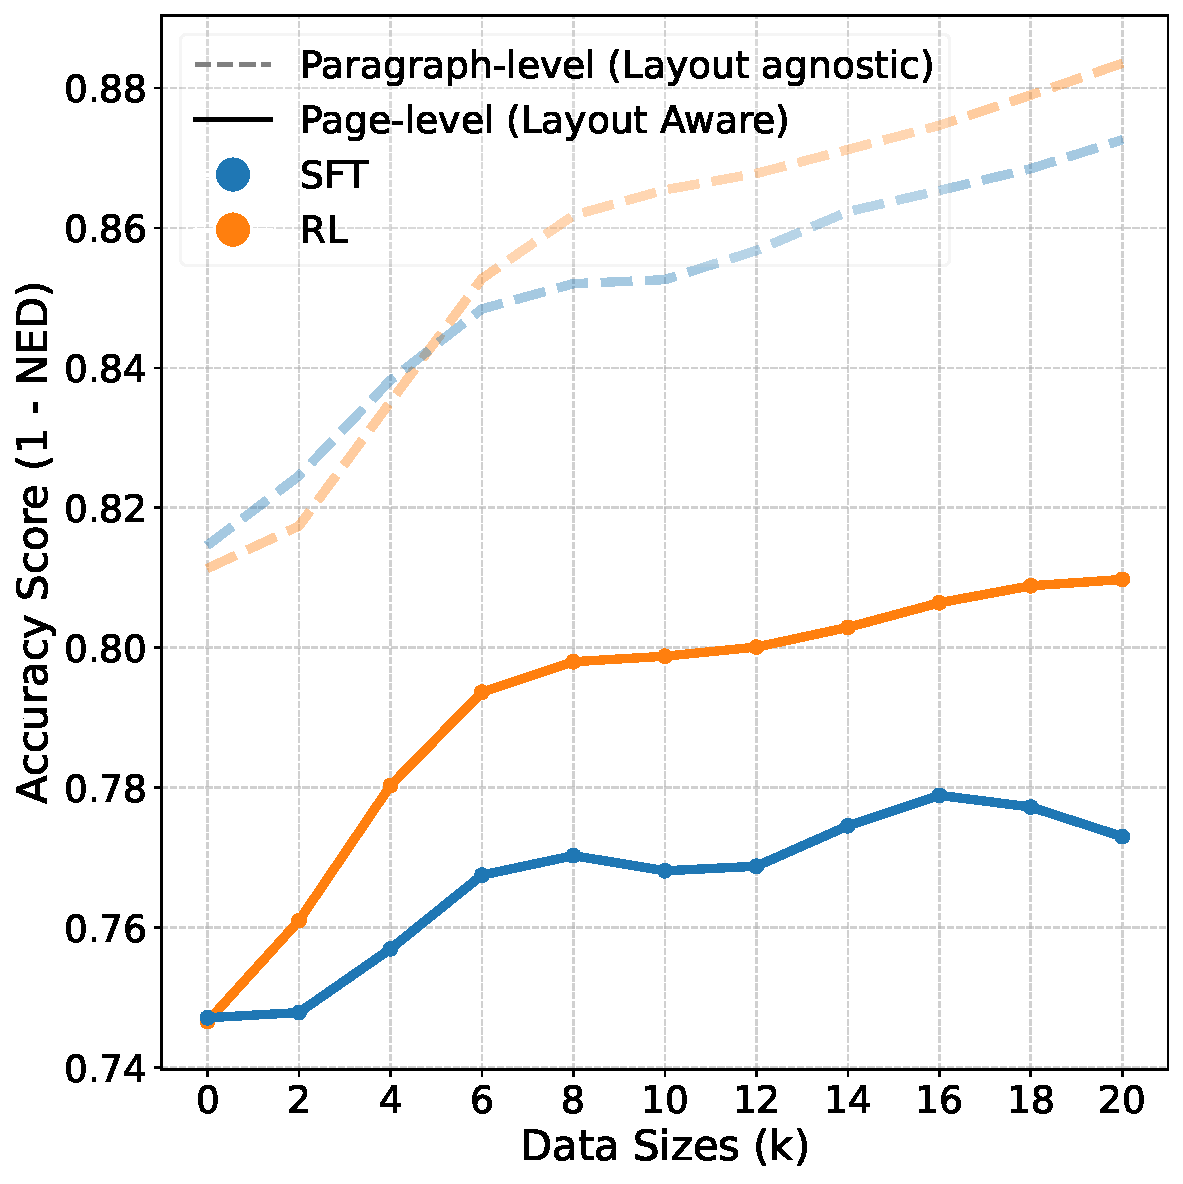
\includegraphics[width=0.48\linewidth]{picture/output_main_with_labels_left_of_end_IID.pdf}
  \hfill
  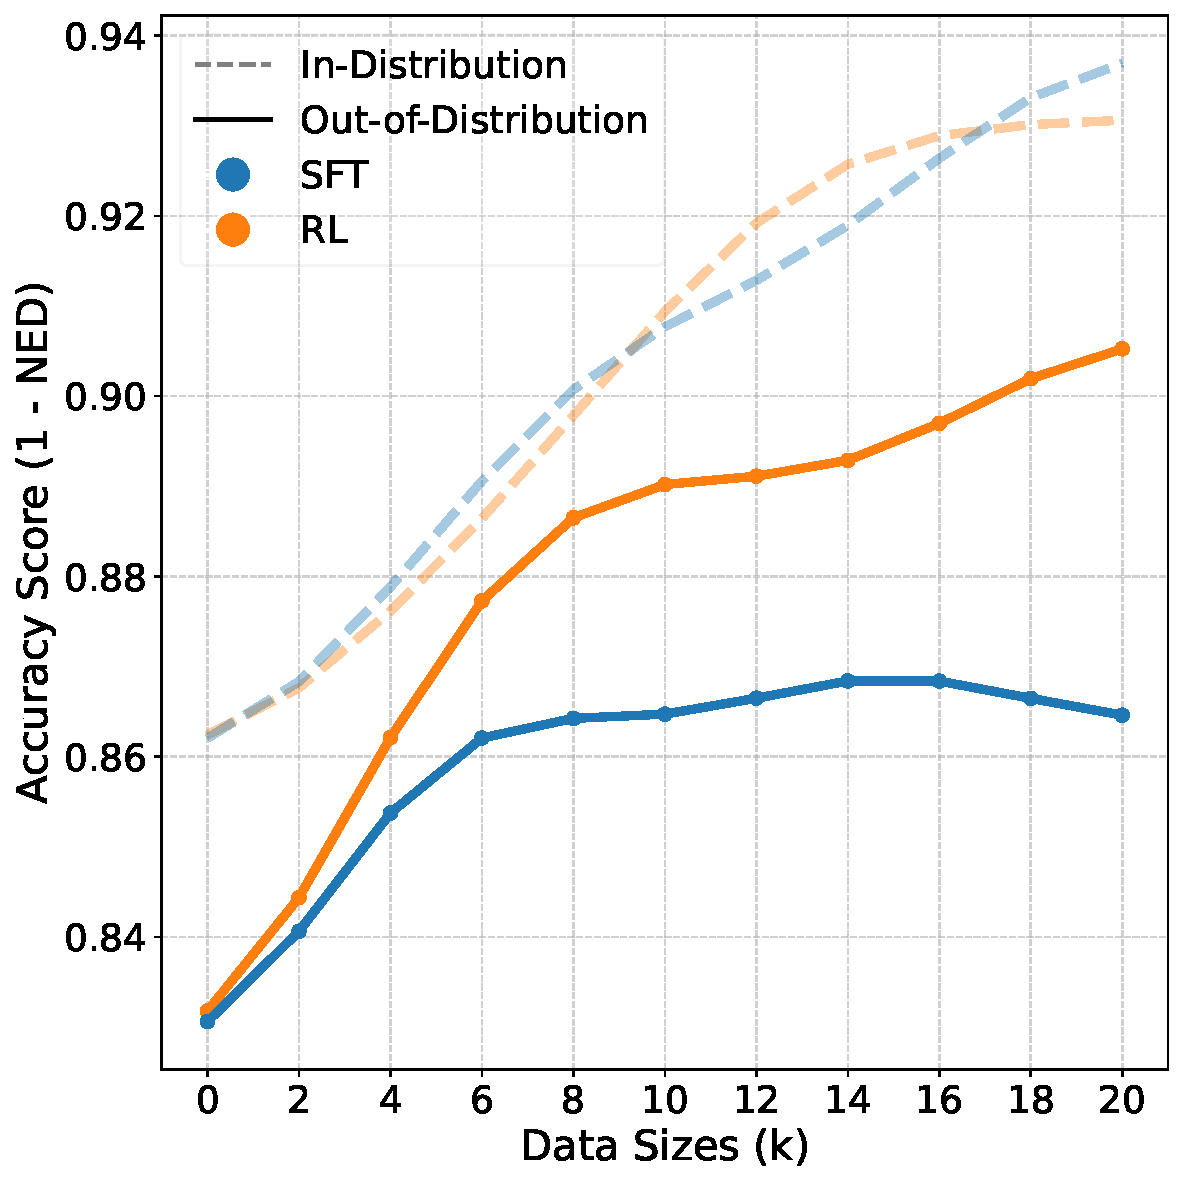
\includegraphics[width=0.48\linewidth]{picture/output_main_with_labels_left_of_end_OOD.pdf}
  \vspace{-2mm}
 \caption{Comparison of document parsing performance on OmniDocBench under different training strategies as training data size increases. Left:  Evaluation with two complementary metrics: (1) Paragraph-level accuracy (edit distance evaluation on element contents only), which assesses element-wise consistency within individual element contents, independent of inter-element reading order; and (2) Page-level accuracy (edit distance evaluation on element contents and reading order), which measures global document reconstruction quality by aligning predicted outputs (e.g., texts, tables, and formulas) with ground-truth sequences. Right: In-Distribution and Out-of-Distribution task performance measured by accuracy score (1 -- NED). See detailed descriptions of the task in Section~\ref{subsec:further_analysis}.}
  \label{fig:example1223xx}
  \vspace{-5mm}
\end{figure}




% To address these limitations, we propose LayoutRL, the first end-to-end reinforcement learning framework that makes document parsers explicitly layout-aware, and construct a new dataset, as shown in Figure 1. 

To address the challenge of effectively applying RL algorithms to document parsing tasks and the lack of large-scale, high-quality data in industry to support this training process, we propose LayoutRL, the first end-to-end reinforcement learning framework for layout-aware document parsing, and construct Infinity-Doc-400K, a large-scale dataset. Specifically, our approach does not rely on explicit reasoning processes, but rather treats the entire document parsing result as the final answer and guides model learning through carefully designed reward mechanisms. We introduce verifiable rewards~\citep{shen2025vlm,liu2024deepseek,shao2024deepseekmath,zheng2025easyr1}, which consist of Edit Distance Reward~\citep{levenshtein1966binary} and Layout Parsing Reward signals, enforcing fine-grained alignment between predictions and ground-truth layouts and providing document-level supervision beyond token-level signals to encourage the model to learn transferable structural representations. Additionally, we construct a 400K-document corpus providing large-scale, high-quality supervision. It combines (1) high-fidelity synthetic scanned document parsing data—generated via HTML templates and browser rendering—and (2) expert-filtered real-world samples, pseudo-labeled through a cross-model agreement pipeline to capture genuine layout diversity. Built on this dataset, we train Infinity-Parser, an end-to-end VLM-based parser that directly outputs structured document representations.


To demonstrate the effectiveness of our approach, we conduct extensive experiments across multiple document parsing benchmarks. Results in Figure~\ref{fig:example1223xx} show that while SFT achieves strong paragraph-level accuracy, its page-level performance struggles to improve as data size increases, reflecting its tendency to memorize surface patterns rather than model the hierarchical dependencies between document structures and elements. In contrast, our layout-aware reinforcement learning method significantly outperforms SFT in page-level accuracy, while maintaining competitive paragraph-level performance. % and exhibiting smoother, more stable learning curves. 
These findings demonstrate that verifiable, layout-aware rewards enable models to move beyond simple token imitation, achieving consistent improvements in both local detail fidelity and global structural understanding, thereby establishing a more robust paradigm for document parsing. Moreover, our method also exhibits strong generalization to unseen task types in downstream applications. Finally, our method, Infinity-Parser, achieves new state-of-the-art results on four diverse benchmarks—OmniDocBench, olmOCR, PubTabNet, and FinTabNet—highlighting its effectiveness and strong cross-domain generalization.


We make the following contributions:

\begin{itemize}[left=0pt]

    \item We propose LayoutRL, a new reinforcement learning framework for end-to-end scanned document parsing, which explicitly trains models to be layout-aware by optimizing verifiable, multi-aspect rewards. Our multi-aspect reward design combines normalized edit distance, paragraph count accuracy, and reading order preservation, improving structural robustness.
  
    \item We introduce Infinity-Doc-400K, a large-scale dataset of 400,482 scanned documents that combines high-quality synthetic data with diverse real-world samples. The dataset features rich layout variations and comprehensive structural annotations, enabling robust training.
    
    \item We train a VLM based model, Infinity-Parser, which sets new state-of-the-art performance across English and Chinese benchmarks for OCR, table and formula extraction, and reading-order detection—demonstrating substantial gains in both structural fidelity and semantic accuracy over specialist pipelines and general-purpose vision-language models. 
\end{itemize}







% \begin{figure}[t!]
%   \centering
%   \resizebox{1\linewidth}{!}{%
%     \includegraphics{picture/case1_V4.pdf}
%   }
%   \caption{Comparison of four Markdown generation results on a single case, illustrating progressive improvement from direct inference to full reward integration.}
%   \label{fig:example1223}
%   \vspace{-5mm}
% \end{figure}





% We conduct experiments comparing SFT with our layout-aware reinforcement learning approach on multiple document parsing tasks. As shown in Figure~\ref{fig:example1223xx}, qualitative results demonstrate that LayoutRL can accurately capture complex table structures and generate clean formatted outputs. In contrast, SFT, though improved over zero-shot baselines, still suffers from symbol errors and content repetition. Quantitative evaluations further confirm these observations: LayoutRL achieves higher structure-level accuracy than SFT, while also exhibiting more stable learning curves without the large fluctuations observed in SFT training. Importantly, LayoutRL shows consistent advantages across both token-level and structure-level metrics, suggesting that our verifiable rewards help the model excel in both local details and global structure understanding.




% To validate our framework, we conduct extensive experiments across diverse benchmarks, including \textit{OmniDocBench}, \textit{PubTabNet}, and \textit{FinTabNet}. Results show that Infinity-Parser achieves stable and balanced performance on both English and Chinese documents. On the most critical metric, \textit{edit distance}, its performance approaches the upper bound of traditional multi-stage pipelines while maintaining strong structural fidelity. Moreover, Infinity-Parser significantly outperforms existing general-purpose vision-language models and specialist expert models in both overall accuracy and layout consistency. Further ablation studies confirm our design choices: whereas supervised fine-tuning struggles to maintain structural precision as data scale increases, layoutRL with fine-grained rewards yields robust generalization and substantially reduces structural hallucinations. These findings provide strong empirical evidence that layout-aware reinforcement learning is a principled and effective paradigm for high-precision scanned document parsing.


% To validate our framework, we conduct extensive experiments across multiple diverse benchmarks, including OmniDocBench, PubTabNet, and FinTabNet. Results demonstrate that Infinity-Parser achieves stable and balanced performance on both English and Chinese documents. On the most critical metric—edit distance—its performance approaches the upper bound of traditional multi-stage pipelines while maintaining strong structural fidelity. Furthermore, Infinity-Parser significantly outperforms existing general-purpose vision-language models and specialized expert models in overall accuracy and layout consistency. Additional ablation studies validate our design choices: reinforcement learning not only learns generalizable rules, but its in-distribution performance improvements also transfer to unseen rules; in contrast, supervised fine-tuning tends to memorize training patterns and lacks cross-task generalization capabilities. Moreover, experimental results in the vision domain show that reinforcement learning can effectively generalize to out-of-distribution tasks, while supervised fine-tuning continues to exhibit poor performance in visual generalization. These results further validate the robustness and cross-domain transfer capabilities of our approach in multimodal tasks, highlighting the advantages of LayoutRL in achieving high-precision document parsing with strong generalization abilities.


% To address these limitations, we propose layoutRL, the first end-to-end reinforcement-learning framework that makes document parsers explicitly layout-aware, and construct a new dataset, as shown in Figure \ref{fig:example_case}. Specially, first,  we incorporate verifiable rewards~\citep{shen2025vlm,liu2024deepseek,shao2024deepseekmath,zheng2025easyr1} that provide document-level supervision beyond token-level signals, encouraging the model to learn transferable structural representations. Second, to mitigate structural hallucination under complex layouts, we design Edit Distance Reward~\citep{levenshtein1966binary} and Layout Parsing Reward signals, including count and order that enforce fine-grained alignment between predictions and ground-truth layouts, improving layout coherence.  Additionally, to support RL training, we construct Infinity-Doc-400K, a 400K-document corpus providing large-scale, high-quality supervision.. It combines (1) high-fidelity synthetic scanned document parsing data—generated via HTML templates and browser rendering—and (2) expert-filtered real-world samples, pseudo-labeled through a cross-model agreement pipeline to capture genuine layout diversity. Built on this dataset, we train Infinity-Parser, an end-to-end VLM-based parser that directly outputs structured document representations.



% To address these limitations, the emergence of large vision-language models (VLMs) has opened a new direction: shifting from brittle pipelines toward unified, end-to-end document parsers. Yet, how to effectively adapt VLMs for layout-sensitive parsing remains an open question. A central issue lies in the choice of training paradigm. Supervised fine-tuning (SFT) provides strong token-level guidance that stabilizes outputs and enforces instruction following, but it tends to memorize surface patterns rather than acquiring transferable structural principles. This limitation is particularly problematic in document parsing, where even minor token errors—such as a misplaced delimiter—can cascade into severe structural deviations. In contrast, reinforcement learning (RL) optimizes against outcome-driven rewards, encouraging models to capture document-level regularities and layout constraints that generalize across unseen domains. Inspired by findings that “SFT memorizes while RL generalizes” in visual perception tasks~\citep{chu2025sft}, we argue that RL offers the right inductive bias for document parsing. However, current RL methods remain constrained by coarse-grained success signals that lack the fine-grained, layout-aware supervision required for complex documents~\citep{liu2025visual,wang2025visualprm,zhou2025r1-zero,meng2025mm}.

% In this work, we introduce layoutRL, the first end-to-end reinforcement learning framework that makes document parsers explicitly layout-aware. To move beyond coarse-grained objectives, we design fine-grained layout-specific rewards. In particular, we incorporate verifiable rewards~\citep{shen2025vlm,liu2024deepseek,shao2024deepseekmath,zheng2025easyr1} that evaluate document structures at the holistic level, and further introduce Edit Distance Rewards~\citep{levenshtein1966binary} and Layout Parsing Rewards (count and order) that enforce alignment between predicted and ground-truth layouts, mitigating structural hallucinations under complex settings. To support training at scale, we construct Infinity-Doc-55K, a 55K-document corpus combining high-fidelity synthetic scanned data with expert-filtered real-world samples pseudo-labeled through cross-model agreement, capturing genuine layout diversity. Built on this dataset, we train Infinity-Parser, an end-to-end VLM-based parser that directly outputs structured document representations.




% Automating the parsing of scanned documents into structured, machine-readable formats remains a key challenge in Document AI~\citep{DocumentParsing1,MinerU,got2,xia2024docgenome,zhang2024document}. Unlike traditional OCR, which focuses on text extraction, document parsing aims to fully understand and reconstruct the document's structure, including the relationships between paragraphs, headings, tables, and other elements. Scanned documents provide valuable visual cues about layout but lack clear semantic markers for structural boundaries. Traditional approaches use multi-stage pipelines—layout detection, OCR, table and formula recognition—followed by heuristic post-processing, but they suffer from error propagation and limited adaptability. In contrast, recent end-to-end vision-language models (VLMs) map document images directly to structured outputs like Markdown, eliminating intermediate stages and offering greater flexibility across document types~\citep{gemini,GPT4}.

% Despite these advancements, document parsing presents unique structural challenges that make it particularly difficult for current VLM training paradigms. Document structures exhibit strong hierarchical dependencies where the placement of key structural tokens—such as section delimiters, list markers, and table boundaries—determines the interpretation of all subsequent content. A single misplaced delimiter or incorrect hierarchy marker can cascade into systematic structural deviations that render the entire parsing result unusable. Current approaches rely primarily on supervised fine-tuning (SFT), which provides strong token-level supervision but tends to memorize surface patterns without acquiring robust structural understanding. This limitation becomes critical in document parsing, where structural integrity depends on precise coordination between visual layout recognition and hierarchical organization. Recent work demonstrates that reinforcement learning (RL) improves models' underlying visual recognition capabilities, contributing to enhanced generalization in visual domains~\citep{chu2025sft}. This suggests that RL could address the structural challenges of document parsing by optimizing for outcome-driven rewards that encourage models to develop robust layout understanding rather than relying on superficial pattern matching. However, existing RL approaches for document parsing remain underdeveloped, constrained by coarse, binary rewards that fail to provide the fine-grained, layout-aware supervision necessary for complex document structures~\citep{liu2025visual,wang2025visualprm,zhou2025r1-zero,meng2025mm}.






% \begin{figure}[t!]
%   \centering
%   \resizebox{1\linewidth}{!}{%
%     \includegraphics{picture/appendix_colorful_textbook.pdf}
%   }
%   \vspace{-7mm}
%   \caption{Comparison of Markdown extraction from a colorful textbook-style PDF. The figure displays the original illustrated page (a), ground truth annotations (b), and outputs from MinerU, GPT-4o, and Infinity-Parser (c–e). Due to the presence of images, varied fonts, and complex layout, MinerU and GPT-4o introduce issues such as redundant content, missed spacing, and incorrect formatting. In contrast, Infinity-Parser accurately identifies section titles and body text, preserving the structure and semantics of the original content.}
%   \label{fig:example123}
%   \vspace{-5mm}
% \end{figure}




% \begin{figure}[t!]
%   \centering
%   \resizebox{1\linewidth}{!}{%
%     \includegraphics{picture/output_main2.pdf}
%   }
%   \caption{From left to right: (1) Ground truth reference; (2) SFT output, which improves formatting and structure but still shows symbol errors and redundant content; (3) RL output, which produces more accurate and concise content; (4) Quantitative comparison between SFT and RL under varying training computation (GFLOPs), showing trends on edit distance and category similarity metrics.}
%   \label{fig:example1223}
%   \vspace{-3mm}
% \end{figure}



% \begin{figure}[t]
%   \centering
%   \resizebox{1\linewidth}{!}{%
%     \includegraphics{picture/figure1_V2.pdf}
%   }
%   \vspace{-3mm}
%   \caption{Overview of the layout-aware reinforcement learning framework. It includes data preparation, reinforcement finetuning, and reward calculation based on edit distance, count, and order to enhance structural understanding.}
%   \label{fig:example_case}
% \vspace{-3mm}
% \end{figure}


%To address the challenges of limited generalization and structural hallucination in document parsing, we propose Infinity-Parser, an end-to-end VLM for scanned document parsing. Infinity-Parser introduces three key innovations. 






% Recent advances in vision-language models (VLMs) have enabled end-to-end approaches that directly map visual document inputs to layout outputs such as Markdown~\citep{bai2025qwen2,InternVL,xu2024llava,thawakar2025llamav}. However, off-the-shelf pretraining objectives—focused on image–text alignment or language modeling—do not inherently encourage preserving a document’s spatial arrangement or reading order. These approaches simplify traditional multi-stage pipelines and offer new possibilities for document parsing, existing models still struggle to generalize effectively on downstream tasks~\citep{MinerU,got2}. A key reason lies in the fundamental mismatch between pretraining objectives and the structural understanding required for document parsing—most pretraining focuses on image-text alignment and reading comprehension, without optimizing for the structural complexities inherent in documents. Compared to standard text, documents exhibit richer, more intricate layouts, characterized by hierarchical layouts, nested elements, and multimodal content~\citep{huang2023improving,VILA}. This complexity introduces challenges that conventional token-level supervision cannot address: prediction errors on a few critical tokens can propagate into substantial structural deviations, and current methods lack fine-grained, layout-aware signals to guide models toward outputs that are both semantically accurate and structurally faithful~\citep{guo2025deepseek,liu2024deepseek,shao2024deepseekmath}. Recent studies show that reinforcement learning (RL) achieves stronger generalization in rule-based and visual reasoning tasks~\citep{chu2025sft}. Existing RL approaches remain constrained by coarse-grained, binary outcome rewards that fail to provide the fine-grained, layout-aware supervision needed for modeling complex document layouts~\citep{liu2025visual,wang2025visualprm,zhou2025r1-zero,meng2025mm}. Designing effective layout-aware reward functions tailored for document parsing remains an underexplored challenge.